\documentclass[a4paper, 11pt]{report}
\usepackage[top=2.5cm, bottom=1.7cm, left=2cm, right=2cm]{geometry}
\usepackage{graphicx}
\usepackage{booktabs}
\usepackage{url}
\usepackage[english]{babel}
\usepackage[latin1]{inputenc}
\usepackage{hyperref}
\hypersetup{
    colorlinks,
    citecolor=black,
    filecolor=black,
    linkcolor=black,
    urlcolor=black
}
\usepackage{mathenv}
\usepackage{amsmath}
\usepackage{color}
\usepackage{caption}
\usepackage[bottom]{footmisc}
\usepackage{cancel}
\usepackage{multirow}
\usepackage[toc,page]{appendix}

\setlength{\parskip}{1em}
\setlength{\parindent}{0em}

\begin{document}

%Titlepage

\pagenumbering{roman}
\begin{titlepage}

	\centering
	
\includegraphics[width=0.15\textwidth]{figs/image_UC.png}\par\vspace{1cm}
	{\scshape\LARGE Facultad de Ciencias \\ Universidad de Cantabria \par}
	
	\vspace{1.5cm}
	
	%English title
	{\huge\bfseries English title}
	
	\vspace{0.6cm}
		
	%Spanish title
	{\LARGE (T�tulo en espa�ol) \par}
	
	\vspace{3cm}
	{\scshape\Large Trabajo de fin de M�ster \\ para acceder al \par}
	\vspace{0.3cm}
	{\scshape\Large \textbf{M�STER UNIVERSITARIO EN \\ CIENCIA DE DATOS} \par}
	
	\begin{flushright}
	
	\vspace{3cm}
	{\Large Autor : C�dric PRIE�LS\par}
	{\Large Director : Pablo MART�NEZ RUIZ DEL �RBOL\\}
	{\Large Co-director : \\}
	\vspace{0.5cm}
	{\Large Junio 2020\par}
	\vfill
	
	\end{flushright}

\end{titlepage}

%Empty page

\clearpage
\thispagestyle{empty}
\phantom{a}
\vfill
\newpage

%Abstract and keywords

\setcounter{page}{1}

\section*{\huge{Abstract}}


\begin{center}
\textbf{Key words} :
\end{center}

\section*{\huge{Resumen}} 

\begin{center}
\textbf{Palabras claves} : 
\end{center}

\newpage

%Thank you notes

\section*{\huge{Agradecimientos}}


\newpage

%Table of contents

\tableofcontents

\thispagestyle{empty}
\newpage

%Here it starts!
\pagenumbering{arabic}

%Introduction

\chapter{Introduction}

Nowadays, muon tomography is an active field of research since it is a non destructive method allowing to map the inside of large objects difficult and/or dangerous to access, without any contact or damage, and without even having physical access to them. To do so, this technique uses muons, elementary particles similar to electrons but with a much greater mass, which allows them to penetrate much deeper and probe matter in a more efficient way, since they suffer less from the bremsstrahlung radiation affecting all leptons. Such technology is relatively well-know and present several advantages over other techniques such as X-ray imaging since it is globally safe and clean and uses natural radiation, cosmic muons, while providing an excellent penetration in matter in order to study it.

In this particular work, muon tomography will be applied to industry and used in order to probe several kinds of objects, such as pipes. This is the main objective of the company Muon systems, founded in Spain in 2015.

\chapter{Theoretical introduction}

\section{Particle physics}

Particle physics is the field which studies the matter surrounding us, along with the fundamental interactions between the particles. In this context, the Standard Model of particle physics \cite{SM} is nowadays the most accepted mathematical model used to describe the elementary particles and three of the 4 fundamental forces of nature (electromagnetic, weak and strong interactions, while the gravitational interaction is out of reach of this model). Even though quite simple in concept, it has been able to describe most of the phenomena observed in nature so far with an incredible level of precision, and has made a lot of predictions that have now been proven to be true, such as the discovery of the top quark \cite{topQuark} in 1995, the tau neutrino \cite{tauNeutrino} in 2001 and the Higgs boson itself \cite{HiggsDiscovery1, HiggsDiscovery2}, the last mising piece of the Standard Model, annouced at CERN in July 2012. 

According to this model, 12 different fermions (along with their 12 corresponding anti-particles) exist in nature, as shown in Figure~\ref{figure:SMFermions}, most of themactually being unstable. These fermions can be divided into two major and fundamentally different categories, the quarks and the leptons, containing each 6 particles and sensitive to different forces. Even though quite interesting, the quarks do not play a fundamantal role in the muon tomography detailed in this work, so only leptons from now on. In particular, leptons can be divided even more into three different generations of particles, and the muon, one particular lepton belonging to the second family, will be the main focus of this work.

\begin{figure}[htbp]
\begin{center}
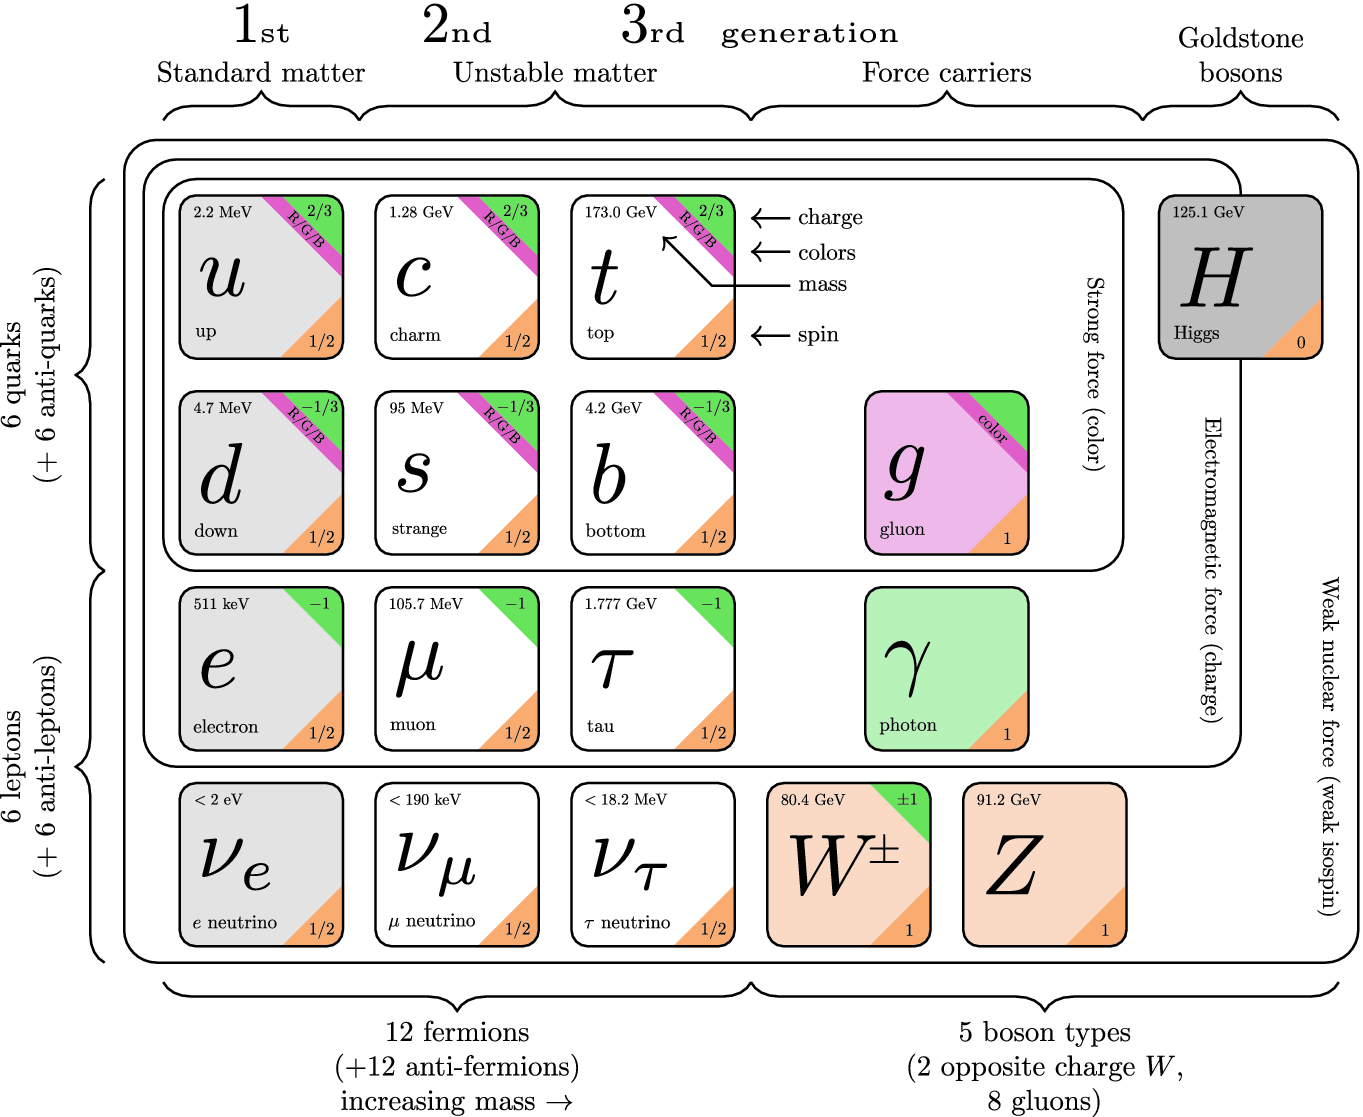
\includegraphics[width=8cm, height=6cm]{figs/SMFermions.png}
\caption{Representation of the 12 fermions of the Standard Model \cite{SMFermions} along with the main force carriers and the Higgs boson, discovered in 2012 and completing this model.}
\label{figure:SMFermions}
\end{center}
\end{figure}

Muons $\mu^{-}$ \cite{PDGMuons} are fundamental particles with a negative charge and quite similar in nature to electrons, even though their high mass (200 times larger than the electron), which implies that their are not stable particles. They actually have a relatively long lifetime of approximately 2.2$\mu$s, and typically decay into an electron while producing two neutrinos in the process. They also have a relatively small interaction cross-section with ordinary matter, even though they do appear with baryonic matter, mostyl due to their electric charge, as will be described in Section~\ref{sec:interactions}.

\section{Cosmic rays}

Being unstable, when produced, muons decay almost instantly into electrons. However, it is possible to observe them in nature, mainly thanks to cosmic rays, constant flux of particles (mostly protons and atomic nuclei) coming from supernovae explosions and AGN emissions and reaching the Earth every day. As they impact our atmosphere, these protons start a chain reactions, as shown in Figure~\ref{figure:cosmic}: first of all, several neutral and charged pions are produced, decaying into a pair of photons (and, later on, the electron and positron pairs) and muons, respectively.

\begin{figure}[htbp]
\begin{center}
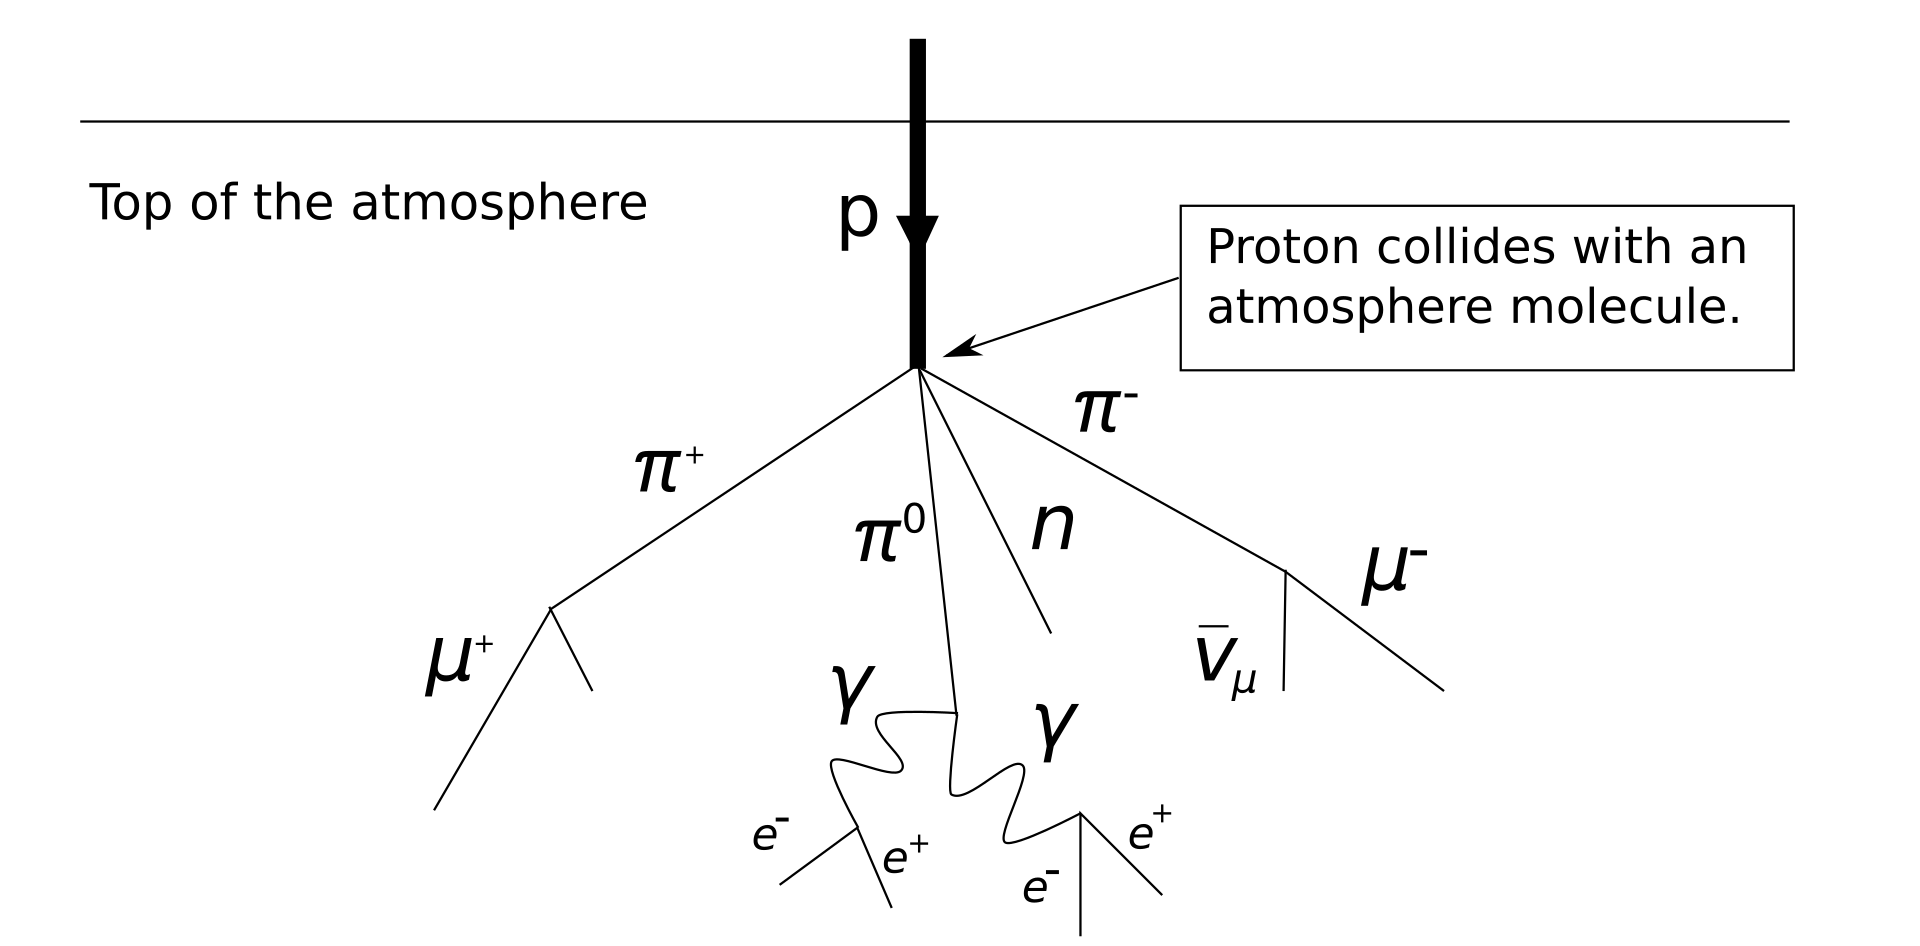
\includegraphics[width=11cm, height=6cm]{figs/cosmic.png}
\caption{Typical chain of reaction induced by a highly energetic cosmic ray when reaching the Earth's atmosphere.}
\label{figure:cosmic}
\end{center}
\end{figure}

Even though the lifetime of muons is quite small, they do manage to reach the sea level thanks to the relatisvistic temporal distorsion induced by their high speed. Muons were actually discovered thanks to cosmic rays in 1936 \cite{muonDiscovery}.

\section{Muons interactions with matter} \label{sec:interactions}
\section{Muon tomography}

These interesting properties can be used in practice.

\chapter{Experimental setup}

\chapter{Code development}

\chapter{Results obtained}

\chapter{Conclusions}

\begin{appendices}
  
  \chapter{Appendix1}
  
\end{appendices}

\addcontentsline{toc}{chapter}{Bibliography}

\begin{thebibliography}{1}

\bibitem{SM}
\href{https://arxiv.org/abs/hep-ph/0510281}{G. Altarelli,
"The Standard Model of Particle Physics",
CERN-PH-TH/2005-206, 2005}

\bibitem{topQuark} 
\href{https://arxiv.org/abs/hep-ex/9503003}{D0 Collaboration,
"Observation of the Top Quark",
Phys.Rev.Lett.74:2632-2637, 1995}

\bibitem{tauNeutrino} 
\href{https://arxiv.org/abs/hep-ex/0012035}{DONUT Collaboration, 
"Observation of Tau Neutrino Interactions",
Phys.Lett.B504:218-224, 2001}

\bibitem{HiggsDiscovery1} 
\href{https://arxiv.org/abs/1207.7235}{S. Chatrchyan et al.,
"Observation of a new boson at a mass of 125 GeV with the CMS experiment at the LHC",
Phys.Lett.B716:30-61, 2012 [arXiv: 1207.7235]
}

\bibitem{HiggsDiscovery2} 
\href{https://arxiv.org/abs/1207.7214}{G. Aad et al.,
"Observation of a new particle in the search for the Standard Model Higgs boson with the ATLAS detector at the LHC", 
Phys.Lett.B716:1-29, 2012 [arXiv: 1207.7214]}

\bibitem{CMS}
\href{http://inspirehep.net/record/796887/}{CMS Collaboration,
"The CMS Experiment at the CERN LHC",
JINST 3 S08004, 2008}

\bibitem{ATLAS}
\href{http://inspirehep.net/record/796888/}{ATLAS Collaboration,
"The ATLAS Experiment at the CERN Large Hadron Collider",
JINST 3 S08003, 2008}

\bibitem{SMFermions}
\href{https://link.springer.com/chapter/10.1007/978-3-030-24370-8_2#citeas}{S. Manzoni, 
"The Standard Model and the Higgs Boson",
Physics with Photons Using the ATLAS Run 2 Data, Springer Theses, 2019
}

\bibitem{PDGMuons}
\href{http://pdg.lbl.gov/2018/listings/rpp2018-list-muon.pdf}{
"Muon", Particle Data Group, 2018}

\bibitem{muonDiscovery}
\href{http://web.ihep.su/dbserv/compas/src/neddermeyer37/eng.pdf}{S.H. Neddermeyer and C.D. Anderson,
"Note on the Nature of Cosmic-Ray Particles", 
Physical Review Vol. 51, 1936}

\end{thebibliography}

\end{document}
